\documentclass{article} % For LaTeX2e
\usepackage{iclr2027_conference,times}

\input{math_commands.tex}

\usepackage{hyperref}
\usepackage{url}
\usepackage{graphicx}
\usepackage{booktabs}
\usepackage{multirow}
\usepackage{amsmath,amssymb}
\usepackage{subcaption}
\usepackage{xcolor}

% Internal revision commands
\newcommand{\todo}[1]{{\color{red}[TODO: #1]}}
\newcommand{\model}{LOCUS}

\title{Scalable Generative Reconstruction of\\Three-Dimensional Fields on Point Clouds}

% Authors hidden for submission; \iclrfinalcopy reveals them.
\author{Nicolas Tricard, Linzheng Wang, Jason Chen, Sili Deng \\
Department of Mechanical Engineering\\
Massachusetts Institute of Technology\\
Cambridge, MA 02139, USA \\
\texttt{\{ntricard,wanglz,jachen25,silideng\}@mit.edu} \\
}

%\iclrfinalcopy % Uncomment for camera-ready version, but NOT for submission.
\begin{document}

\maketitle

\begin{abstract}
Reconstructing three-dimensional physical fields from sparse measurements is an ill-posed inverse problem for which generative models provide the natural formulation: they sample from the posterior over fields rather than regressing to its mean. Current generative reconstruction methods, however, do not survive the transition from two to three dimensions. Voxel-based diffusion models hit a memory wall that has forced published 3D efforts onto cropped subdomains and reduced architectures, while latent-space methods circumvent the cost by compressing fields through an autoencoder, bounding reconstruction by the compression stage and risking the small scales that sparse reconstruction is meant to recover. We introduce \model{}, a conditional rectified-flow model that generates fields directly in ambient function space, on arbitrary point clouds, with no autoencoder and no voxelization. Its velocity network conditions each query point through a compact global summary of the observations and a strictly local, importance-weighted retrieval over sensor tokens, so per-query cost is constant and total cost is linear in the number of points; because the training objective is an integral over the domain, it is estimated on a random subset of points at each step, decoupling training cost from resolution. A single amortized model handles arbitrary sensor counts, layouts, noise levels, and observed-channel patterns at test time. Across isotropic turbulence at two million points, transonic wing aerodynamics on unstructured meshes with surface-only observations, and buoyant fire plumes under noisy and occluded sensing, \model{} is competitive in accuracy with voxel- and latent-space baselines that are locked to their training grids, trains and samples with memory decoupled from output resolution, and---where every scored precedent in the literature is underdispersed---produces the best-calibrated posteriors of any method we evaluate, under proper scoring rules and paired significance tests.
\end{abstract}

\section{Introduction}
\label{sec:intro}

Volumetric fields govern the systems that experiments and monitoring campaigns can only observe pointwise. Particle-image velocimetry resolves planes of a turbulent flow while the surrounding volume remains unmeasured; flight-test and wind-tunnel campaigns record surface pressure at taps while the off-body flow that determines performance is inaccessible; combustion diagnostics image one or two species along a sheet; ocean and atmospheric networks sample tower, buoy, and sonde locations separated by kilometers. Recovering the full three-dimensional state from such measurements is a long-standing inverse problem \citep{callaham2019robust,raissi2020hidden,vinuesa2023transformative}, and at realistic sensor densities it is severely ill-posed: many fields are consistent with the data, and the missing information resides disproportionately at the small scales. Deterministic reconstruction networks \citep{fukami2021global,santos2023senseiver,dang2025flronet} return a conditional mean, which is the optimal point estimate and also a systematically over-smoothed one; the estimate blurs precisely the fine-scale structure whose recovery motivates reconstruction in the first place. Generative models resolve this mismatch by sampling from the posterior over fields given the observations, retaining sharp realizations and quantifying what the measurements do not determine \citep{shu2023physics,li2024s3gm,zhuang2025spatially}.

This posterior-sampling program has largely been carried out in two dimensions. Guided diffusion reconstructs 2D turbulence from sparse pixels \citep{shu2023physics,amoros2026guiding}, pretrained score models assimilate sparse observations of 2D dynamics zero-shot \citep{li2024s3gm,huang2024diffusionpde}, and amortized conditional diffusion handles moving sensor arrays on 2D grids \citep{zhuang2025spatially}. In parallel, a line of work has moved generative modeling from fixed grids to function space, defining diffusions and flows over functions so that training and sampling are consistent across discretizations \citep{kerrigan2024functional,lim2025score,pidstrigach2024infinite,shi2025stochastic}, with guided variants for inverse problems \citep{yao2025fundps,kerrigan2024dynamic}. These methods establish the right abstraction for measurements that arrive at scattered locations, but their demonstrations remain at $64\times64$ to $128\times128$ resolution on uniform 2D grids, with spectral backbones that presuppose those grids; scaling guided function-space sampling beyond two dimensions is stated as an open problem \citep{yao2025fundps}.

The transition to three dimensions has instead been attempted along two detours, each with a documented cost. The first is voxelization. Dense 3D U-Nets and transformers compute globally on the full grid at every training step, so activation memory grows with the cube of resolution: published 3D generative models cap their domains at $192\times48\times48$ \citep{lienen2024zero}, train on $32^3$ crops with attention removed to avoid out-of-memory failures \citep{oommen2026turbulent}, restrict attention to factorized axes at $64^3$ \citep{li2023factformer}, or build dedicated patch-decomposition pipelines because full-volume training at $512^3$ is infeasible \citep{holzschuh2026pd3}. Voxelization also forfeits the geometry: unstructured simulation meshes and scattered sensors must be resampled onto axis-aligned grids before any of these models apply. The second detour is latent compression. Autoencoding the field into a compact code and running diffusion or flow matching in the code space \citep{du2024confild,zhou2025text2pde,wang2026fundiff,li2025latent} makes 3D generation affordable, but the reconstruction quality is bounded by the autoencoder, and this bound is not tight enough for turbulence: mean-squared-error-trained autoencoders retain roughly a quarter of the spectral power in the dissipation range \citep{rafiq2026spectrally}, convolutional compression of 3D turbulence degrades high-wavenumber content \citep{glaws2020deep}, and latent neural-field models report systematic small-scale and near-wall discrepancies on their own benchmarks \citep{du2024confild}. A generative reconstructor whose prior cannot represent the small scales cannot return them in its posterior, whatever the observations. Meanwhile, the architectures that do scale to realistic 3D discretizations---transformer surrogates operating on millions of mesh points \citep{luo2025transolver,alkin2024upt,alkin2025abupt,li2023gino}---are uniformly deterministic; generative modeling on meshes and point clouds has been limited to a few thousand nodes \citep{lino2025dgn}. The combination that practice requires, a generative model that samples full 3D fields on arbitrary point sets at realistic resolution, is absent from the literature.

A further gap separates published evaluations from deployed sensing. The dominant protocol conditions on noiseless values subsampled from simulation output at freely chosen interior locations \citep{shu2023physics,huang2024diffusionpde,amoros2026guiding}. Deployed measurements are noisy, are frequently confined to surfaces \citep{guastoni2021convolutional,cuellar2024three,mousavi2025low}, suffer occlusion from the phenomena being measured, and often observe different physical quantities than the ones of interest, as when planar species imaging must stand in for velocity or temperature in a flame \citep{barwey2021extracting,kildare2024deep}. These conditions are not corner cases; they define the regime in which reconstruction is used. They are also the regime in which the generative formulation earns its cost: with noiseless, well-placed observations, deterministic models are competitive \citep{zhuang2025spatially}, and benchmarks restricted to that setting understate the gap that opens once noise and ambiguity are present.

We introduce \model{}, a generative reconstruction model designed for this regime. \model{} performs conditional rectified flow directly on field values evaluated at scattered spatial points---ambient space, end to end, with no autoencoder and no voxel grid---with a Gaussian-process source distribution that ties the pointwise flow into a coherent flow over functions. Tractability at scale follows from two architectural decisions. First, conditioning is factored by locality: a cross-attention encoder compresses the sensor set into a compact global summary at cost linear in the number of sensors, and each query point retrieves a small, importance-weighted neighborhood of sensor tokens through a learned distance metric, at constant cost per query. The velocity network therefore never forms a global volumetric representation, and its total cost is linear in the number of evaluation points with no all-to-all term. Second, because the flow-matching objective is an integral over the domain, it admits unbiased estimation on random subsets of points: \model{} trains on roughly one percent of the discretization per step, which decouples training memory from resolution. Neither decision is available to a voxel U-Net or a patchified transformer, whose computation graphs are global in the discretization. Conditioning is amortized over randomized sensor configurations during training, so a single model serves arbitrary sensor counts, placements, noise levels, and observed-channel subsets at test time, and rectified flow yields usable posterior samples in as few as two to sixteen network evaluations.

Our contributions are as follows.
\begin{itemize}
\item We present the first generative model that reconstructs three-dimensional physical fields at realistic discretization sizes directly in ambient function space, combining locality-factored conditioning with subsampled function-space training; we show that this combination, and not raw architecture capacity, is what removes the 3D memory wall (Section~\ref{sec:results-scaling}).
\item On forced isotropic turbulence at two million points per snapshot, \model{} trains on a single GPU at full resolution, where voxel diffusion and patchified-transformer baselines exceed memory or require crops, and it preserves dissipation-range spectra that a parameter-matched latent flow-matching baseline truncates (Section~\ref{sec:results-scaling}).
\item On transonic wing aerodynamics over varying geometries, \model{} operates natively on unstructured RANS meshes and infers volumetric flow posteriors from surface-only observations, a measurement operator that grid-based generative baselines cannot represent without resampling (Section~\ref{sec:results-geometry}).
\item Under noisy, occluded, and cross-variable measurement operators on buoyant fire-plume LES data, \model{} degrades gracefully and produces calibrated posterior spreads, while deterministic point-cloud baselines collapse to over-smoothed means and voxel baselines inherit their resolution limits (Sections~\ref{sec:results-realism} and~\ref{sec:results-crossvar}).
\end{itemize}

\section{Related Work}
\label{sec:related}

\paragraph{Sparse field reconstruction.}
Deterministic learned reconstruction spans convolutional models on Voronoi-embedded sensor images \citep{fukami2021global}, attention over arbitrary sensor sets with coordinate-query decoding \citep{santos2023senseiver}, operator-learning hybrids \citep{dang2025flronet}, and shallow decoders for fixed arrays \citep{erichson2020shallow}. Wall-to-volume estimation has been studied with convolutional networks and GANs under fully resolved wall fields \citep{guastoni2021convolutional,cuellar2024three}, and low-order estimators with uncertainty from sparse noisy taps \citep{mousavi2025low}. These models handle flexible sensing but return point estimates; under severe ill-posedness they regress toward the conditional mean and lose small-scale structure. Classical assimilation and physics-informed approaches \citep{raissi2020hidden,cai2021flow} recover fields per case through optimization and do not amortize across conditions.

\paragraph{Generative reconstruction.}
Diffusion models condition on sparse observations through guidance at sampling time \citep{shu2023physics,huang2024diffusionpde,amoros2026guiding,chung2023diffusion,rozet2023score}, through pretrained unconditional models with assimilation-style sampling \citep{li2024s3gm}, or through amortized conditional training \citep{zhuang2025spatially,liu2024uncertainty}. Nearly all of this work operates on uniform 2D grids. The 3D exceptions illustrate the cost of the voxel route: crops, reduced architectures, and capped domains \citep{oommen2026turbulent,lienen2024zero}. Latent-space generative reconstruction \citep{du2024confild,zhou2025text2pde,lino2025dgn} extends to irregular domains through neural-field or graph decoders but inherits the autoencoder's spectral floor \citep{rafiq2026spectrally,glaws2020deep} and, in the graph case, has been demonstrated only at thousands of nodes \citep{lino2025dgn}. \model{} differs from all of these in generating directly in ambient space on the measurement discretization, with amortized conditioning and no compression stage.

\paragraph{Probabilistic evaluation of reconstruction.}
Although the generative reconstruction literature routinely draws posterior ensembles, it almost never scores them. Across the conditional-generative sparse-sensor reconstruction methods we surveyed, evaluation stops at pointwise error and physics statistics; ensembles appear as mean-and-spread figures, and several works claim calibrated uncertainty on the evidence of standard-deviation maps alone \citep{wang2025geofunflow}. Proper scoring rules and calibration diagnostics \citep{gneiting2007strictly} enter only at the margins of the field: a latent-diffusion reconstruction of the atmospheric boundary layer reports a rank histogram and finds its ensemble underdispersed \citep{rybchuk2023ensemble}; kilometer-scale generative weather assimilation scores CRPS and spread--skill and likewise finds miscalibration \citep{manshausen2025generative}; graph-diffusion urban assimilation reports CRPS on a single fixed geometry \citep{giral2026genda}; and sensor-time-history decoders report CRPS and coverage for 2D slices \citep{gao2026uqshred}. Flow-matching reconstruction with ``quantified uncertainty'' on wall-bounded turbulence reports spread maps and spectra but no score \citep{parikh2026conditional}, and set-conditioned flow matching for sparse inversion reports only a variance--error correlation \citep{yang2025pis}. To our knowledge, no prior work demonstrates a \emph{calibrated} posterior for three-dimensional field reconstruction from scattered point sensors under a proper scoring rule; every scored precedent, in any adjacent setting, is underdispersed. We therefore report fair CRPS, spread--error ratios, central-interval coverage, and rank histograms for our model and for every baseline capable of producing an ensemble, with paired per-snapshot significance tests.

\paragraph{Generative models in function space.}
Score-based diffusion and flow matching have been lifted to function spaces with well-posedness guarantees \citep{lim2025score,pidstrigach2024infinite,kerrigan2024functional,franzese2023continuous}, extended to stochastic-process priors and functional regression \citep{shi2024universal,shi2025stochastic}, and applied to inverse problems through function-space guidance \citep{yao2025fundps,baldassari2023conditional,kerrigan2024dynamic}. Physics-oriented instantiations include function autoencoders with latent diffusion \citep{wang2026fundiff} and subsampled-state image diffusion \citep{bond2024infty}. The demonstrations are one- and two-dimensional at moderate resolution, typically with FFT-based backbones tied to uniform grids, and guidance-based conditioning multiplies sampling cost. \model{} keeps the function-space formulation---coordinates in, field values out, a smooth Gaussian-process source, resolution-independent training---while replacing the spectral backbone with a point-cloud architecture that scales to 3D and replacing test-time guidance with amortized conditioning.

\paragraph{Scaling field models to 3D and point clouds.}
Deterministic surrogates have scaled to large unstructured discretizations through graph message passing \citep{pfaff2021learning}, linear-attention operators \citep{hao2023gnot,wu2024transolver}, latent-grid operators \citep{li2023gino}, and hierarchical or anchored attention reaching millions of points \citep{luo2025transolver,alkin2024upt,alkin2025abupt}. This line establishes that locality and factorized attention, not dense global computation, are what scale; none of it is generative. On the generative side, 3D voxel diffusion remains resolution-capped \citep{lienen2024zero,li2023factformer,holzschuh2026pd3}, and mesh-based generative models remain small \citep{lino2025dgn}. \model{} transfers the scaling ingredients of the deterministic line into a conditional flow-matching model, which requires the conditioning pathway itself, not only the backbone, to be local and linear.

\section{Method}
\label{sec:method}

\subsection{Problem setup}
\label{sec:method-setup}

Let $u:\Omega\to\R^{C}$ denote a physical field on a spatial domain $\Omega\subset\R^{d}$ with $d=3$, drawn from an underlying distribution over fields (snapshots of a turbulent flow, converged RANS solutions over varying geometry and flight condition). The field is observed through a measurement operator that returns a finite set of scalar readings
\begin{equation}
\mathcal{O}=\{(\vx_j,\,c_j,\,y_j)\}_{j=1}^{M},\qquad y_j = u_{c_j}(\vx_j)+\varepsilon_j,
\label{eq:obs}
\end{equation}
where $\vx_j\in\Omega$ is a sensor location, $c_j$ indexes the observed quantity, and $\varepsilon_j$ is sensor noise. This formulation covers the sensing conditions that motivate this work: the locations $\vx_j$ may be scattered arbitrarily or confined to a surface $\partial\Omega_b\subset\Omega$; the observed quantities $c_j$ may cover only a subset of the target channels, or quantities that are not target channels at all (wall shear stress observed while volumetric velocity is sought); and known scalar covariates such as the freestream Mach number enter simply as additional tokens in $\mathcal{O}$. The goal is to sample from the posterior $p(u\mid\mathcal{O})$, evaluated at an arbitrary finite set of query locations $\{\vy_i\}_{i=1}^{N}$ that need not coincide with any training discretization.

\subsection{Rectified flow on point sets with a Gaussian-process source}
\label{sec:method-flow}

\model{} models the conditional distribution with a rectified flow \citep{liu2023flow,lipman2023flow,albergo2023building} defined directly on field values. The source distribution is a Gaussian process rather than pointwise white noise: a draw $u_0\sim\pi_0$ evaluated at coordinates $\{\vy_i\}$ is produced by a random-feature expansion \citep{rahimi2007random},
\begin{equation}
u_0(\vy) = \sqrt{\tfrac{2}{F}}\,\sum_{f=1}^{F} w_f \cos\!\big(\boldsymbol{\omega}_f^{\top}\vy+b_f\big),\qquad w_f\sim\gN(0,1),
\label{eq:rff}
\end{equation}
with frequencies $\boldsymbol{\omega}_f$ drawn once from a Gaussian whose scale sets the prior correlation length. Evaluating \eqref{eq:rff} at any two point sets yields marginals of one consistent function-valued source, which is what makes training and sampling coherent across discretizations: the same model can be trained on one point subset and sampled on another, denser one. Given a data field $u_1$ evaluated at the same points, the state interpolates linearly, $u_t=(1-t)\,u_0+t\,u_1$, and a velocity network $v_\theta$ is trained to regress the constant displacement:
\begin{equation}
\gL(\theta)=\E_{t,\,u_0,\,u_1,\,\mathcal{O}}\ \frac{1}{|\Omega|}\int_{\Omega}\big\| v_\theta\big(t,\,u_t(\vy),\,\vy;\,\mathcal{O}\big)-\big(u_1(\vy)-u_0(\vy)\big)\big\|_2^2\, d\vy .
\label{eq:loss}
\end{equation}
The objective is an integral over the domain, and this is the property that removes the resolution barrier: \eqref{eq:loss} admits an unbiased Monte Carlo estimate over a random subset of query points at every step. In practice \model{} trains on roughly $1\%$ of the available discretization per step ($1.9\times10^{4}$ of $1.95\times10^{6}$ points on the turbulence benchmark), so training memory is set by the subset size, not the resolution. Voxel U-Nets, latent autoencoders, and patchified transformers do not admit this estimator; their computation graphs couple all grid locations, and their training cost is tied to the full resolution regardless of the loss. Sampling integrates the learned ODE from a fresh source draw with a uniform Euler scheme; because rectified-flow paths are near-straight, $2$--$16$ network evaluations suffice, compared with the hundreds to thousands used by guided diffusion \citep{li2024s3gm,huang2024diffusionpde}. Posterior diversity comes from the source draw: repeated integration under the same $\mathcal{O}$ yields an ensemble.

\begin{figure}[t]
\begin{center}
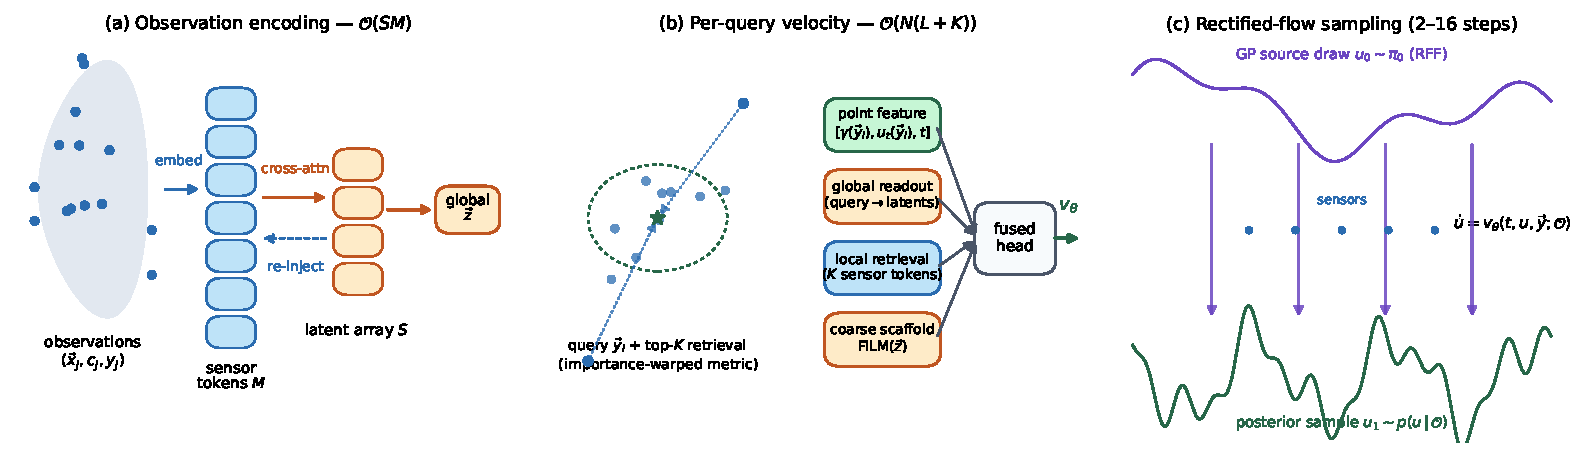
\includegraphics[width=\linewidth]{figures/architecture.pdf}
\end{center}
\caption{\textbf{The \model{} architecture.} Observations are embedded as sensor tokens and compressed by cross-attention into a small latent array (global pathway, $\gO(SM)$), which re-injects context back into the sensor tokens. Each query point assembles its velocity from three sources: its own point features, a readout from the latent array, and an importance-weighted retrieval over its $K$ nearest sensor tokens under a learned, importance-warped metric (local pathway, $\gO(NK)$). No dense volumetric representation is ever formed; total cost is linear in the number of query points. Training estimates the flow-matching loss on a random $\sim$1\% subset of points per step.}
\label{fig:architecture}
\end{figure}

\subsection{Locality-factored conditioning}
\label{sec:method-arch}

The velocity network must expose the observations to every query point without incurring an all-to-all term in $N$ or a dense volumetric representation. \model{} factors the conditioning pathway by locality (Figure~\ref{fig:architecture}).

\paragraph{Sensor tokens and global summary.}
Each observation $(\vx_j,c_j,y_j)$ is embedded as a token from a Fourier positional encoding of $\vx_j$ \citep{tancik2020fourier}, the reading $y_j$, and a learned embedding of the quantity index $c_j$. A small array of $S$ learnable latents cross-attends to the $M$ sensor tokens \citep{jaegle2021perceiver}, at cost $\gO(SM)$, and is refined by self-attention blocks that re-attend to the sensor tokens between rounds, so the compact summary can resolve detail where sensors are dense. The mean-pooled latent array provides a global summary vector $\vz$; a second cross-attention pass writes the refined global context back into the individual sensor tokens, giving each sensor a representation of its measurement in context.

\paragraph{Per-query velocity assembly.}
For a query $\vy_i$, three components are fused. (i) A point feature encodes the positional embedding of $\vy_i$, the current state $u_t(\vy_i)$, and $t$. (ii) A global readout cross-attends from a coordinate-conditioned decoder token to the latent array, at cost $\gO(L)$ per query. (iii) A local retrieval gathers the $K$ nearest sensor tokens under an importance-warped metric
\begin{equation}
d(\vy_i,\vx_j)^2=\|\vy_i-\vx_j\|_2^2 - \beta_j,
\label{eq:metric}
\end{equation}
where $\beta_j$ is a learned per-sensor importance bias predicted from the sensor token, and combines them with normalized RBF weights. The bias lets informative sensors extend their influence beyond their Euclidean neighborhood, which matters when sensing is anisotropic (surface-only layouts) or partially corrupted. A FiLM-modulated coarse prediction from the global summary is added as a gated residual, anchoring the local estimate in the system-scale structure. The fused representation passes through a small MLP head to the velocity. The retrieval and the $k$-nearest-neighbor search are evaluated with streaming kernel reductions \citep{charlier2021kernel}, so the $[N{\times}M]$ distance matrix is never materialized. Total cost per network evaluation is $\gO(SM + NL + NK)$ with no term coupling query points to each other: memory and compute are linear in $N$, and the same trained network evaluates on $10^{4}$ or $2\times10^{6}$ points unchanged.

\subsection{Amortized measurement operators}
\label{sec:method-operators}

Conditioning is amortized by randomizing the measurement operator during training. Each step draws the sensor count and layout afresh; with configurable probability, readings are corrupted with Gaussian noise of random amplitude, contiguous sensor regions are removed (slab or ball occlusions), and entire observed channels are dropped. The network therefore learns a single conditional velocity field over a family of operators, and at test time one model serves arbitrary layouts, counts, noise levels, and observed-channel patterns without retraining or guidance. Known covariates (Mach number, angle of attack) are appended as parameter tokens with dedicated quantity indices, exempt from corruption. At sampling time, observed values can additionally be enforced on the generated field, either by overwriting at sensor locations after each step or through a clean-endpoint blending schedule; we use hard enforcement for noiseless protocols and disable it under sensor noise, where exact interpolation of corrupted readings is not desirable. Training details, including the bf16 setting and the weight-averaging used for evaluation, are given in Appendix~\ref{app:training}.

\section{Experiments}
\label{sec:results}

\paragraph{Datasets.}
Three domains, chosen so that each exposes one failure mode of existing methods. (i) Forced isotropic turbulence from the Johns Hopkins Turbulence Database \citep{li2008public}: a $125^3$ cutout of the $1024^3$ DNS ($1.95\times10^{6}$ points per snapshot; velocity and pressure; 617 snapshots, 555/62 split). (ii) SHIFT-WING \citep{luminary2026shiftwing}: adaptively meshed RANS solutions over parametric variants of the NASA CRM wing--fuselage at transonic conditions; we use 222 cases (200/22 split), each reduced to $4\times10^{5}$ near-body volume mesh nodes and $6.5\times10^{4}$ surface nodes carrying pressure and wall shear stress. Geometry varies across cases and enters only through the observation point cloud; Mach number and angle of attack enter as parameter tokens. (iii) FireBench \citep{firebench2024}: a large-eddy simulation of wildfire spread; we extract a 3D fire-front region ($3.7\times10^{6}$ points; velocity, potential temperature, fuel density; 22 snapshots) from the public store.

\paragraph{Baselines.}
We compare against the three routes to 3D generative reconstruction identified in Section~\ref{sec:intro}, each parameter-matched where applicable. The latent route: a 3D convolutional autoencoder with rectified flow in its latent space (LDM-style \citep{rombach2022high}, conditioned on rasterized sensor masks), trained end to end on the same data. The voxel route: SiT-style transformers with patchified tokenization \citep{ma2024sit,peebles2023dit} and guided voxel diffusion with hard observation masking \citep{amoros2026guiding}, trained at the largest resolution that fits in memory, with crops where required---resolution ceilings are reported as results, not hidden. The deterministic point-cloud route: Senseiver \citep{santos2023senseiver}, the strongest published attention-based sparse reconstructor, trained with the identical sensor randomization. CoNFiLD \citep{du2024confild} provides an external latent-neural-field comparison. \todo{Finalize CoNFiLD adaptation and per-dataset baseline coverage table.}

\paragraph{Metrics.}
Accuracy: relative $L_2$ of the posterior mean and of single samples. Spectral fidelity: shell-averaged energy spectra, log-spectral distance, and band-resolved energy errors (large/medium/dissipation scales). Distributional fidelity: cross-channel joint PDFs with Jensen--Shannon divergence. Probabilistic calibration, computed from $K$-member ensembles: fair CRPS \citep{gneiting2007strictly}, spread--error ratio, central-interval coverage, and rank histograms. Cost: peak training memory and wall-clock versus resolution and query count.

\subsection{The 3D memory wall and spectral fidelity: isotropic turbulence at two million points}
\label{sec:results-scaling}
\todo{JHU results: accuracy vs baselines table; memory/wall-clock scaling curves vs resolution (LOCUS linear, voxel cubic, patchify token blowup); spectra + band-resolved errors vs latent-FM AE floor; NFE sweep (2--16); query-subsampling ablation.}

\subsection{Irregular geometry and surface-only observation: transonic wing aerodynamics}
\label{sec:results-geometry}
\todo{SHIFT-WING results: volumetric posterior from 128--4096 surface taps across geometries; comparison to Senseiver and latent baselines (voxel methods inapplicable without resampling -- state explicitly); midspan slice galleries; tap-count scaling; posterior std concentrating at shock/wake.}

\subsection{Realistic measurement operators: noise, occlusion, and calibration}
\label{sec:results-realism}
\todo{JHU-robust + FireBench: noise sweeps (0--0.3 std), slab/ball occlusions, tower-layout zero-shot transfer; calibration metrics vs deterministic mean-collapse; robust-trained vs clean-trained model.}

\subsection{Cross-variable inference}
\label{sec:results-crossvar}
\todo{FireBench: wind-only observations -> temperature/fuel-density posterior (fire-front localization); JHU: velocity -> pressure; joint PDFs + JSD; enabled by channel-dropout amortization.}

\subsection{The 3D memory wall and spectral fidelity: isotropic turbulence at two million points}
\label{sec:results-scaling}
\todo{JHU isotropic1024 cutout results: accuracy vs baselines, memory/wall-clock scaling curves, spectra and band-resolved errors, NFE sweep, query-subsampling ablation.}

\subsection{Irregular geometry and surface-only observation: transonic wing aerodynamics}
\label{sec:results-geometry}
\todo{SHIFT-WING results: volumetric posterior from surface sensors across geometries; comparison to Senseiver/GINO-style and latent baselines; qualitative fields on unstructured meshes.}

\subsection{Realistic measurement operators: noise, occlusion, and calibration}
\label{sec:results-realism}
\todo{FireBench results: noise sweeps, occlusion masks, calibration metrics, deterministic mean-collapse comparison.}

\subsection{Cross-variable inference}
\label{sec:results-crossvar}
\todo{Observed-channel transfer: velocity-only observations inferring temperature/scalars and vice versa; joint PDFs and JSD.}

\section{Conclusion}
\label{sec:conclusion}

Generative reconstruction of three-dimensional fields has been blocked not by modeling capacity but by a structural mismatch: the architectures used for generation compute globally on dense discretizations, while the problem is defined on scattered points and demands only local and summary information at each of them. \model{} resolves the mismatch by carrying flow matching directly on field values with a Gaussian-process source, factoring conditioning into a compact global summary and importance-weighted local retrieval, and estimating the training objective on random point subsets. The result is a single amortized model that trains at two-million-point resolution on one GPU, operates natively on unstructured meshes and surface-only sensing, and returns posterior ensembles under noise and occlusion where deterministic surrogates collapse to the mean. \todo{Sharpen with final numbers; add limitations (temporal dynamics out of scope here, calibration gap, per-domain training) and outlook (forecasting extension, cross-domain pretraining, experimental data).}

\subsection*{Reproducibility statement}
All experiments use publicly available data: the JHTDB isotropic turbulence database, the SHIFT-WING dataset (CC-BY-NC-4.0), and the public FireBench store; exact cutout indices, crop definitions, subsampling seeds, and normalization are specified in Appendix~\ref{app:datasets}. Architecture and training hyperparameters for \model{} and all baselines are listed in Appendices~\ref{app:architecture}--\ref{app:baselines} together with the configuration files used for every run. Code, configurations, and dataset preparation scripts will be released. \todo{Anonymous code link at submission.}

\subsection*{AI use statement}
\todo{Complete per ICLR 2027 policy before submission: disclose the use of AI assistance for literature search, code development, and manuscript drafting, with author verification of all content.}

\bibliography{references}
\bibliographystyle{iclr2027_conference}

\appendix
\section{Training details}
\label{app:training}
\todo{Optimizer, schedules, bf16 autocast, EMA, per-dataset hyperparameters, hardware, wall-clock budgets.}

\section{Architecture details}
\label{app:architecture}
\todo{Layer dimensions, attention configuration, importance-bias parameterization, kNN backend, chunking.}

\section{Datasets and preprocessing}
\label{app:datasets}
\todo{JHU cutout construction; SHIFT-WING crop/subsampling/nondimensionalization; FireBench subset; splits.}

\section{Baseline configurations}
\label{app:baselines}
\todo{Latent flow matching (ConvAE3D + latent U-Net), voxel guided diffusion, SiT, Senseiver, CoNFiLD; parameter budgets and training protocols.}

\section{Additional results}
\label{app:results}
\todo{Extra fields, extra metrics, per-snapshot distributions, qualitative galleries.}

\end{document}
